% C3E --- npj Digital Medicine submission build.
%
% One of three builds. ../main.tex is the full-length venue-neutral draft and is
% never compressed; ../jamia/ is the JAMIA fallback; this is the primary target.
% Each venue build owns its own sections/ copies because the three restructure
% the same material differently and cannot share files.
%
% Requirements from the official npj submission guide
% (nature.com/documents/npj-submission-guide.pdf), Article content type:
%
%   Abstract        ~150 words, UNSTRUCTURED and unreferenced
%   Main text       5,000 words
%   Methods         separate from the main-text count; typically <= 3,000,
%                   "may be longer if necessary"
%   Display items   10 --- figures and tables COMBINED, not 4 + 6
%   References      usually up to 70
%   Title           <= 15 words, no punctuation, no abbreviations, no active verbs
%   Headings        "Avoid 'Introduction' as a heading". Subheadings belong
%                   mainly in Results.
%   Order           abstract, unheaded opening, Results, Discussion, METHODS,
%                   Data Availability, References
%
% The Methods-excluded main-text budget is why this build has far less to cut
% than the JAMIA one: 5,000 words of main text plus a separately counted Methods,
% against JAMIA's 4,000 for everything.
%
% Build:  cd paper/npjdm && latexmk -pdf main_npjdm.tex
% Budget: ./budget.sh

\documentclass[11pt,a4paper]{article}

\usepackage[utf8]{inputenc}
\usepackage[T1]{fontenc}
\usepackage{lmodern}
\usepackage[margin=1in]{geometry}
\usepackage{amsmath,amssymb}
\usepackage{booktabs}
\usepackage{multirow}
\usepackage{graphicx}
\usepackage{siunitx}
\usepackage[hidelinks]{hyperref}
\usepackage[capitalise,noabbrev]{cleveref}
\usepackage{xcolor}
\usepackage{setspace}
\usepackage[modulo]{lineno}

% npj is flexible about initial-submission formatting ("style and length will not
% influence consideration"), but line numbers and generous spacing make a
% reviewer's job easier and cost nothing.
\onehalfspacing
\linenumbers

\graphicspath{{../}{./}}

\sisetup{detect-weight=true, group-minimum-digits=4, group-separator={,}}

\newcommand{\overbudget}[1]{%
  \par\medskip\noindent\fcolorbox{orange!60}{orange!5}{%
    \parbox{0.95\linewidth}{\small\textbf{OVER BUDGET:} #1}}\par\medskip}

\date{}

\begin{document}

% ---------------------------------------------------------------------------
% Title. npj asks for 15 words or fewer, with no punctuation and no active
% verbs -- which rules out the question form used by the venue-neutral draft
% and the JAMIA build ("Does multimodal selective reliability transport across
% hospitals when pre-diagnostic clinical context changes?", 17 words, a
% question mark and an active verb). Recast as a noun phrase, 13 words.
% ALTERNATIVE, if the two findings should be given equal billing:
%   "Label dependence and non-transport of frozen selective-prediction policies
%    across hospitals" (10 words)
% ---------------------------------------------------------------------------
\begin{center}
{\LARGE\bfseries Non-transport of a frozen multimodal selective-prediction
policy across hospitals under compound context shift\par}

\vspace{1.5em}

{\large Shakib Howlader\textsuperscript{1,*} \quad
Adnan Rahman Sayeem\textsuperscript{1}\par}

\vspace{1em}

\begin{singlespace}
\textsuperscript{1}[DEPARTMENT], Daffodil International University, Dhaka,
Bangladesh\\
\textsuperscript{*}Corresponding author: [INSTITUTIONAL EMAIL]
\end{singlespace}
\end{center}

\vspace{2em}

% ---------------------------------------------------------------------------
% Abstract. npj wants roughly 150 words, unstructured and unreferenced: a
% general introduction to the topic, then a non-technical summary of the main
% results and their implication. This is NOT the JAMIA structured abstract --
% do not paste that one in.
% ---------------------------------------------------------------------------
\begin{abstract}
\noindent
Selective prediction lets a chest-radiograph model defer uncertain cases to a
radiologist, and the abstention threshold that fixes its operating point is
chosen once, at the hospital where the model was built. We report a
preregistered evaluation of whether that frozen policy survives deployment
elsewhere, while the pre-diagnostic clinical context such models consume also
changes. Models developed on one hospital's radiographs were evaluated at a
second with every threshold transferred unchanged, under context left intact,
removed, or replaced with another patient's. The policy did not transport:
selective error rose several times above the prespecified materiality while
realised coverage stayed within its drift tolerance --- a degradation invisible
to coverage monitoring, and erased rather than repaired by re-calibrating at
the receiving site. A prespecified label-source sensitivity then reversed every
cross-site contrast while leaving within-site contrasts intact, establishing
that the two automatically derived label sets are not commensurable across
these cohorts.
\end{abstract}

\clearpage

% ---------------------------------------------------------------------------
% Main text. Opens without a heading, per Nature style.
% ---------------------------------------------------------------------------
% Nature style: the main text opens without a heading. npj: "Avoid
% 'Introduction' as a heading." Do not add one.


A chest-radiograph classifier that knows when to defer is more useful in a
hospital than one that is merely accurate. Selective prediction formalises
this: the model returns a decision only when its confidence clears a threshold,
and refers the remainder to a human reader. The threshold fixes an operating
point --- a coverage --- and with it the workload the system imposes on
radiology.

That operating point is chosen once, on data from the hospital where the system
was developed. It is then deployed somewhere else. Whether it survives the move
is an empirical question that is rarely asked, and the way it is usually asked
answers something narrower than intended: models are re-evaluated at a second
site, but the abstention threshold is re-fitted there too. A re-fitted threshold
tests whether a \emph{method} transfers. It cannot test whether a \emph{deployed
policy} transfers, because the policy that would actually ship is the frozen
one.

A second shift travels with the first and is usually left implicit. Multimodal
chest-radiograph models increasingly consume clinical context alongside the
image --- the indication, the referring history, the reason the study was
ordered. This text is not a stable input. Its availability is a property of how
a particular hospital documents care, and it varies across institutions in ways
that have nothing to do with the patient. A model that learned to lean on the
indication field at one site may find it thin, absent, or differently written at
the next.

Institution and context therefore shift together. Studies that vary one hold the
other fixed: cross-institution work is typically image-only, and multimodal
context work is typically single-institution. Holding one fixed cannot reveal
whether they interact, and interaction is precisely what determines deployment
risk. If a multimodal model is more accurate at the source site \emph{because}
of context, and context is scarcer at the target site, then the measured benefit
and the unmeasured fragility are the same phenomenon observed from two sides.

This paper contributes an evaluation protocol that crosses the two shifts
deliberately, so their interaction can be estimated rather than assumed away:

\begin{itemize}
  \item \textbf{Two sites.} A source hospital, where models are developed and
    the selective policy is calibrated, and an external hospital used only for
    evaluation.
  \item \textbf{Three controlled context states at each site.} Context left
    intact, context removed, and context replaced with another patient's ---
    the last separating \emph{absence} of information from \emph{wrong}
    information.
  \item \textbf{A frozen policy.} Per-pathology thresholds and abstention
    cutoffs are selected once at the source site and transferred unchanged, so
    what is evaluated is the policy that would actually ship.
  \item \textbf{Preregistration} in a machine-readable, hash-manifested
    protocol, with every amendment dated and its confirmatory status recorded,
    so the boundary between prespecified and post-hoc is auditable rather than
    asserted.
\end{itemize}

The contribution is the protocol and what it measures. We propose no new
architecture and no new uncertainty algorithm; the backbones are deliberately
conventional, held constant so that architecture cannot serve as a competing
explanation for any effect observed. This is not a prospective clinical study or
a regulatory validation.

Two further contributions emerged from building the protocol and are reported
because they generalise beyond it. First, a structural hazard in deriving
pre-diagnostic context from radiology reports: a substantial minority of reports
embed a preliminary interpretation inside the report body, so any pipeline that
takes ``everything before the findings section'' as context silently ingests
post-diagnostic text (\cref{sec:report-structure}). Second, a property of the
decision rule this literature commonly uses --- requiring both that a confidence
interval exclude zero and that the point estimate reach a materiality threshold
--- which caps statistical power at \SI{50}{\percent} when the true effect
equals that threshold, regardless of sample size (\cref{sec:power}).

\label{sec:related-work}

Every work cited here was verified against its official publication page or
full text.

\paragraph{Selective prediction under distribution shift}

Selective classification has been extended to distribution shift outside
medicine. The closest methodological work generalises selective classification
so that a model rejects not only ambiguous in-distribution inputs but
label-shifted and covariate-shifted ones, using margin-based confidence scores
requiring no access to training data, evaluated on ImageNet, ImageNet-C,
OpenImage-O, iWildCam, Amazon and CIFAR~\cite{selective_shift_2025}.

That line establishes the machinery this paper applies. It does not take it to a
clinical setting, does not involve a second hospital, and does not transfer a
threshold frozen at one site to another. Whether an abstention policy remains at
its intended operating point after institutional transfer is not addressed
there, and is the question we ask.

\paragraph{Clinical context as a model input}
\label{sec:rw-context}

Clinical history improves chest-radiograph classification. The most directly
comparable work fuses view-specific image encoders with clinical history through
an attention-refinement mechanism on MIMIC-CXR-JPG, reporting
\num{135682} images with clinical history alongside a further \num{59846}
without~\cite{yang2025mcxnet}.

That paper is a premise for ours rather than a competitor, and the distinction
is worth stating precisely. It is single-institution, evaluated on held-out
splits of one source, with no abstention policy, no audit of whether the
diagnosis leaks into the history text, and no calibration transfer. Its
\num{59846} context-free images are an \emph{observation} of naturally occurring
missingness. We \emph{intervene} on context under a frozen informativeness rule,
which is what allows an effect to be attributed to the manipulation rather than
to whatever else distinguishes patients whose indication field happens to be
empty.

A second study reaches the same conclusion by a different route, fusing
multi-view radiographs with clinical indications and vital signs and reporting
an ablation in which each added modality
contributes~\cite{sloan2025clinically}. That ablation is additive: it measures
what each modality contributes as the model is built. Ours is interventional: it
measures what a fixed, already-trained model loses when context degrades at
deployment. The distinction is not pedantic, since a component that improves a
model during development need not be one whose absence degrades it
proportionally afterwards, and only the second quantity bears on deployment
risk. That work also evaluates on benchmark splits of a single source, with no
second institution, no abstention, and no threshold transfer.

\paragraph{Missing modalities as an architectural problem}

A body of work treats missing modalities as something to engineer around.
Transformer-based bi-modal fusion modules combined into a tri-modal framework,
trained with multivariate losses for robustness to missing modalities on a
14-label diagnosis task over MIMIC-IV and MIMIC-CXR, is
representative~\cite{wang2025missing}; so is a mixture-of-experts framework
selecting experts according to which modalities are present, for mortality,
length-of-stay and readmission prediction~\cite{wang2025moehealth}.

The orientation differs from ours in a way that matters. There, missingness is
an obstacle and robustness is the objective; the natural question is how to keep
performance up when a modality drops out. Here, missingness is the
\emph{estimand}. We do not ask how to build a model that resists context loss,
but how much reliability a conventionally built model loses when context
degrades, and whether that loss is larger at a hospital the model has never
seen. Both approaches also evaluate within a single source, so neither can speak
to transfer.

\paragraph{Cross-institution generalisation in chest radiography}

Cross-domain generalisation for chest-radiograph models is well studied.
Foundational work across multiple datasets argues that cross-domain failure is
driven by label shift rather than image shift, observing that models with strong
individual performance disagree substantially with one
another~\cite{cohen2020limits}. More recent multi-center benchmarking over
\num{145000} images from PadChest and NIH Chest X-ray evaluates head-versus-tail
performance, calibration and cross-center generalisation gaps, and concludes
that detecting rare findings under multi-center shift remains
challenging~\cite{cxrlt2026}.

A related strand examines robustness to technical acquisition parameters rather
than to institution. Comparing four architectures for the sensitivity gap
between anteroposterior and posteroanterior views, model rankings reverse
completely on a second dataset: a chest-radiograph-specific vision-language
model with the smallest internal gap (\SI{14.3}{\percent}) shows the largest
external one (\SI{48.9}{\percent}), while a self-supervised model stays near
its internal value~\cite{farquhar2026acquisition}. That the second dataset
shares an institution with the first, differing principally in labelling
convention, makes the reversal more striking rather than less: internal ranking
failed to predict external ranking without a change of hospital at all.

This line is image-only. It varies institution, acquisition, or labelling while
holding input availability fixed --- the mirror image of
\cref{sec:rw-context} --- and none of it evaluates abstention or transfers a
threshold frozen. Thresholds are re-fitted per dataset, typically by Youden's
statistic, so what is measured is whether a method can be re-tuned rather than
whether a policy survives the move. That the most recent multi-center benchmark
still names calibration and cross-center generalisation as open problems
supports treating the crossed question as unresolved rather than answered
piecemeal.

\paragraph{The gap}

Each axis has been studied in isolation: selective prediction under shift
outside medicine~\cite{selective_shift_2025}; clinical context helping within a
single hospital~\cite{yang2025mcxnet,sloan2025clinically}; missing modalities
handled architecturally within a single
source~\cite{wang2025missing,wang2025moehealth}; institutional, acquisition and
labelling shift characterised for image-only
models~\cite{cohen2020limits,cxrlt2026,farquhar2026acquisition}.

Absent is the crossing: an evaluation in which institution and pre-diagnostic
context availability vary together, under a selective policy frozen at the
source site and transferred without refitting, with the interaction estimated
rather than assumed. That is the design this paper specifies and reports.

\section{Results}
\label{sec:results}

All estimates are selective five-label Hamming error at the frozen
\SI{80}{\percent} coverage cutoff, with \SI{95}{\percent} percentile intervals
from a patient-clustered bootstrap of \num{2000} replicates. Thresholds and
abstention cutoffs are the source-site values applied unchanged at both sites.
This section reports what was estimated; interpretation is deferred to
\cref{sec:discussion}.

\begin{figure}[tbp]
\centering
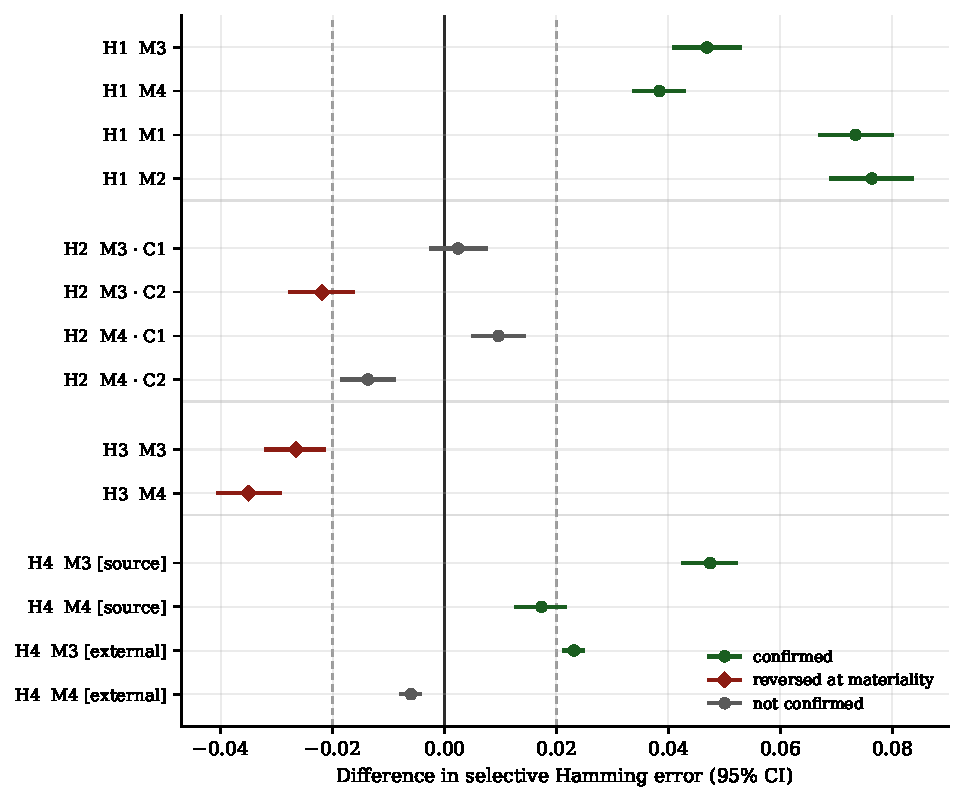
\includegraphics[width=\linewidth]{figures/fig1_forest}
\caption{Confirmatory contrasts with \SI{95}{\percent} percentile intervals
from the patient-clustered bootstrap. Dashed lines mark the materiality
threshold of $\pm\num{0.02}$. Two contrasts are reversed: their intervals
exclude zero on the side opposite the prediction, with magnitudes exceeding
materiality.}
\label{fig:forest}
\end{figure}

\cref{fig:forest} summarises the four confirmatory contrasts; the
subsections below give the estimates.

\subsection{Cohorts}

The source confirmatory tier comprises \num{16456} images from \num{14766}
studies and \num{5000} patients. Every study is informative (N1) by
construction, since cohort selection already required context above the frozen
threshold.

The external cohort comprises \num{191070} usable images from \num{187673}
studies and \num{64709} patients, one image having been excluded as corrupt in
the published dataset. Here the natural-state distribution is informative:
\num{132923} studies (\SI{70.8}{\percent}) are N1, \num{14129}
(\SI{7.5}{\percent}) are N2, and \num{40622} (\SI{21.6}{\percent}) are N3.
Interventions therefore apply to \num{132923} external studies against
\num{14766} source studies.

Invariants held at both sites. Image-only predictions were identical across all
three context conditions (maximum drift \num{0}), and studies retaining their
own context under C2 numbered \num{6} of \num{14766} at the source site and
\num{34} of \num{132923} at the external site.

\subsection{Selective risk at both sites}

\begin{table}[htbp]
\centering
\caption{Selective Hamming error at the frozen \SI{80}{\percent} cutoff. M1 is
image-only, M2 text-only, M3 probability late fusion, M4 feature-concatenation
fusion. M1 is invariant to the context intervention by construction.}
\label{tab:selective-risk}
\begin{tabular}{lccc c ccc}
\toprule
& \multicolumn{3}{c}{Source site} & & \multicolumn{3}{c}{External site} \\
\cmidrule{2-4}\cmidrule{6-8}
Model & C0 & C1 & C2 & & C0 & C1 & C2 \\
\midrule
M1 & 0.1084 & 0.1084 & 0.1084 & & 0.1818 & 0.1818 & 0.1818 \\
M2 & 0.1575 & 0.2411 & 0.2415 & & 0.2338 & 0.2605 & 0.2667 \\
M3 & 0.1102 & 0.0951 & 0.1426 & & 0.1570 & 0.1444 & 0.1676 \\
M4 & \textbf{0.0744} & 0.0720 & 0.0893 & & \textbf{0.1128} & 0.1200 & 0.1140 \\
\bottomrule
\end{tabular}
\end{table}

M4 attains the lowest selective error under every site-by-condition
combination (\cref{fig:risk}).

\begin{figure}[htbp]
\centering
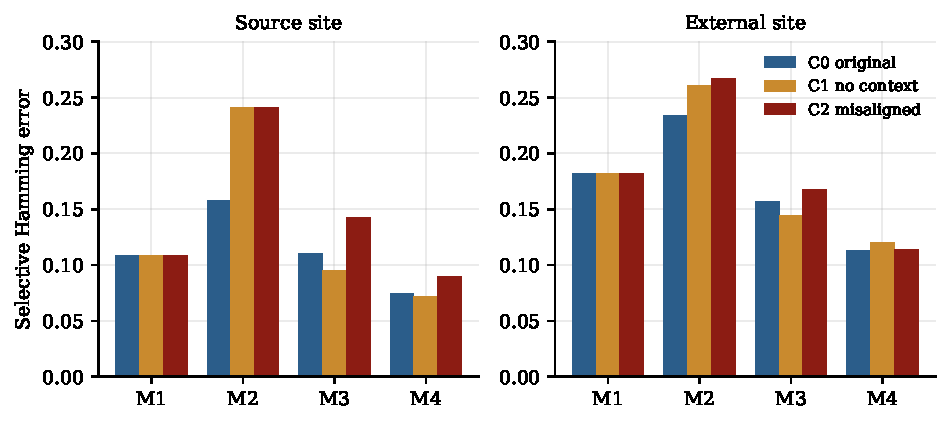
\includegraphics[width=\linewidth]{figures/fig2_risk}
\caption{Selective Hamming error at the frozen \SI{80}{\percent} cutoff.
Every model degrades on institutional transfer; the ordering between models is
preserved.}
\label{fig:risk}
\end{figure}


\subsection{H1: transport of the selective policy}

\begin{table}[htbp]
\centering
\caption{H1, external minus source selective error under intact context (C0).
M3 and M4 are the confirmatory models; M1 and M2 are reported for context.}
\label{tab:h1}
\begin{tabular}{lccl}
\toprule
Model & Estimate & \SI{95}{\percent} CI & Verdict \\
\midrule
M3 & $+0.0469$ & $(+0.0408,\ +0.0531)$ & \textbf{confirmed} \\
M4 & $+0.0384$ & $(+0.0336,\ +0.0430)$ & \textbf{confirmed} \\
\midrule
M1 & $+0.0734$ & $(+0.0668,\ +0.0802)$ & confirmed \\
M2 & $+0.0763$ & $(+0.0687,\ +0.0838)$ & confirmed \\
\bottomrule
\end{tabular}
\end{table}

H1 is confirmed for both confirmatory models. Every interval excludes zero in
the hypothesised direction and every point estimate exceeds the materiality
threshold of \num{0.02}, by factors of \numrange{1.9}{3.8}. These estimates are
taken under C0, with context intact at both sites.

\subsection{H2: compound interaction}

\begin{table}[htbp]
\centering
\caption{H2, the interaction between institutional and context shift, computed
as the context effect at the external site minus the same effect at the source
site. A positive value would indicate super-additivity.}
\label{tab:h2}
\begin{tabular}{llcl}
\toprule
Model & Condition & Estimate & \SI{95}{\percent} CI \\
\midrule
M3 & C1 & $+0.0024$ & $(-0.0027,\ +0.0076)$ \\
M3 & C2 & $-0.0219$ & $(-0.0279,\ -0.0160)$ \\
M4 & C1 & $+0.0096$ & $(+0.0048,\ +0.0144)$ \\
M4 & C2 & $-0.0137$ & $(-0.0185,\ -0.0087)$ \\
\bottomrule
\end{tabular}
\end{table}

H2 is not confirmed in any of its four instances. One estimate is
indistinguishable from zero (M3 under C1). Two exclude zero in the direction
opposite to the hypothesis (M3 and M4 under C2), and for M3 the magnitude
reaches materiality, so the effect is reversed rather than absent. The
remaining estimate excludes zero in the hypothesised direction but falls below
materiality (M4 under C1, $+0.0096$).

\subsection{H3: multimodal versus image-only exposure}

\begin{table}[htbp]
\centering
\caption{H3, the transfer gap of each multimodal model minus the transfer gap of
the image-only control. A positive value would indicate greater multimodal
exposure.}
\label{tab:h3}
\begin{tabular}{lccl}
\toprule
Contrast & Estimate & \SI{95}{\percent} CI & Verdict \\
\midrule
M3 $-$ M1 & $-0.0265$ & $(-0.0321,\ -0.0212)$ & reversed at materiality \\
M4 $-$ M1 & $-0.0350$ & $(-0.0408,\ -0.0292)$ & reversed at materiality \\
\bottomrule
\end{tabular}
\end{table}

H3 is not confirmed, and the direction is reversed for both models. Each
interval lies entirely below zero, and each magnitude exceeds materiality.
Both multimodal models carry smaller transfer gaps than the image-only control.
The advantage of M4 over M1 in absolute selective error also widens across
sites, from \num{0.034} at the source site to \num{0.069} at the external site.

\subsection{H4: conflicting versus absent context}

\begin{table}[htbp]
\centering
\caption{H4, C2 minus C1 within site. A non-negative value indicates that
misaligned context is no better than absent context.}
\label{tab:h4}
\begin{tabular}{llccl}
\toprule
Site & Model & Estimate & \SI{95}{\percent} CI & Verdict \\
\midrule
Source   & M3 & $+0.0475$ & $(+0.0422,\ +0.0524)$ & confirmed \\
Source   & M4 & $+0.0173$ & $(+0.0125,\ +0.0217)$ & confirmed \\
External & M3 & $+0.0231$ & $(+0.0211,\ +0.0250)$ & confirmed \\
External & M4 & $-0.0060$ & $(-0.0080,\ -0.0041)$ & not confirmed \\
\bottomrule
\end{tabular}
\end{table}

H4 holds in three of four instances. The exception is M4 at the external site,
where the estimate is negative and its interval excludes zero, but the
magnitude is below materiality.

\subsection{Coverage under the frozen cutoff}

A coverage drift of \num{0.05} from the \SI{80}{\percent} target was
prespecified as material. Under intact context, no model breaches it at either
site; the largest external departure is M2 at $+0.0469$ and the smallest is M4
at $-0.0051$.

Four breaches occur, all under context intervention and all at both sites
alike:

\begin{itemize}
  \item M2 under C1 reaches \SI{100}{\percent} coverage at both sites
    (drift $+0.20$). Replacing every context with a single placeholder makes the
    text-only model's output constant, so all studies clear the confidence
    cutoff simultaneously.
  \item M3 under C2 falls to \SI{72.8}{\percent} at the source site
    (drift $-0.0718$) and \SI{74.6}{\percent} at the external site
    (drift $-0.0537$).
\end{itemize}

M4's coverage remains within \num{0.036} of target under every site-by-condition
combination.

\begin{figure}[htbp]
\centering
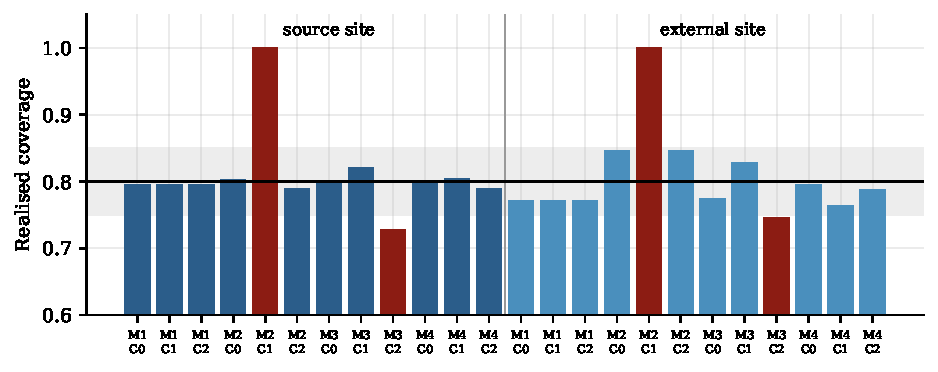
\includegraphics[width=\linewidth]{figures/fig3_coverage}
\caption{Realised coverage under the frozen cutoff. The shaded band marks the
prespecified material drift of \num{0.05} either side of the
\SI{80}{\percent} target; bars breaching it are darkened. Coverage survives
institutional transfer and fails under context intervention.}
\label{fig:coverage}
\end{figure}

\subsection{Coverage sensitivity}

Coverages of \SI{90}{\percent} and \SI{70}{\percent} were pre-specified as
sensitivity analyses alongside the primary \SI{80}{\percent}.

\begin{table}[htbp]
\centering
\caption{Point estimates for the two confirmatory contrasts across the three
pre-specified coverages. H1 is the transfer gap under intact context; H3 is that
gap minus the image-only control's.}
\label{tab:coverage-sensitivity}
\begin{tabular}{llccc}
\toprule
& Model & \SI{70}{\percent} & \SI{80}{\percent} & \SI{90}{\percent} \\
\midrule
\multirow{2}{*}{H1} & M3 & $+0.0394$ & $+0.0469$ & $+0.0548$ \\
                    & M4 & $+0.0392$ & $+0.0384$ & $+0.0374$ \\
\midrule
\multirow{2}{*}{H3} & M3 & $-0.0296$ & $-0.0265$ & $-0.0234$ \\
                    & M4 & $-0.0299$ & $-0.0350$ & $-0.0408$ \\
\bottomrule
\end{tabular}
\end{table}

Both conclusions hold across all three coverages. Every H1 estimate remains
positive and above materiality, and every H3 estimate remains negative and above
materiality in magnitude, so neither the confirmation nor the reversal depends on
the choice of operating point. The two multimodal models respond to coverage in
opposite directions --- M3's transfer gap grows with coverage while M4's shrinks
--- but not enough to alter either verdict.

\subsection{Informativeness-threshold sensitivity}
\label{sec:threshold-sensitivity}

A study enters the intervention cohort as N1 only if its pre-diagnostic context
carries at least $T$ effective tokens. $T = 3$ was pre-specified as primary;
$T = 5$ and $T = 10$ were pre-specified as sensitivities. The threshold is a
cohort definition rather than a model setting, so raising it does not merely
perturb an estimate --- it re-runs the whole evaluation on a smaller and more
text-rich population. At the external site the N1 cohort falls from
\num{132923} studies at $T = 3$ to \num{111040} at $T = 5$ and \num{23146} at
$T = 10$, the last retaining under a fifth of the primary cohort; at the source
site it falls from \num{14766} to \num{13600} and \num{8381}. Studies leaving N1
become N2, so the comparison is between populations, not nested subsamples of
one.

\begin{table}[htbp]
\centering
\caption{Point estimates for the two confirmatory contrasts across the three
pre-specified informativeness thresholds, at \SI{80}{\percent} coverage. H1 is
the transfer gap under intact context; H3 is that gap minus the image-only
control's.}
\label{tab:threshold-sensitivity}
\begin{tabular}{llccc}
\toprule
& Model & $T = 3$ & $T = 5$ & $T = 10$ \\
\midrule
\multirow{2}{*}{H1} & M3 & $+0.0469$ & $+0.0381$ & $+0.0221$ \\
                    & M4 & $+0.0384$ & $+0.0330$ & $+0.0232$ \\
\midrule
\multirow{2}{*}{H3} & M3 & $-0.0265$ & $-0.0314$ & $-0.0338$ \\
                    & M4 & $-0.0350$ & $-0.0366$ & $-0.0327$ \\
\bottomrule
\end{tabular}
\end{table}

All fourteen contrasts --- the four confirmatory ones and the ten secondary and
descriptive ones --- return the same verdict at every threshold. Both H1
estimates stay positive and above materiality, and both H3 estimates stay
negative and above materiality in magnitude, so neither the confirmation of H1
nor the reversal of H3 depends on where the informativeness cut is placed.

The two hypotheses respond to the threshold in opposite directions, and the
direction is interpretable. H1's transfer gap shrinks as $T$ rises, roughly
halving for M3 between $T = 3$ and $T = 10$: restricting the cohort to studies
with substantial context reduces, but does not remove, the penalty for moving
sites. H3's reversal instead deepens slightly, so the multimodal models'
advantage over the image-only control is not an artifact of admitting
thin-context studies that the fusion models handle better than M1 does.

One interval changes character without changing a verdict. H4 for M4 at the
external site is $-0.0060$ (\SI{95}{\percent} CI \numrange{-0.0080}{-0.0041}) at
$T = 3$ but $-0.0020$ ($-0.0067$ to $+0.0023$) at $T = 10$, crossing zero as the
cohort shrinks to \num{23146} studies. The verdict is unaffected because the
estimate falls far short of the \num{0.02} materiality threshold at every $T$
and was never confirmed, but the widening is the expected consequence of a
five-fold smaller cohort and is reported rather than suppressed.

\subsection{S1: cross-site contrasts are not label-invariant}
\label{sec:s1}

The findings-derived label source was pre-specified as a mandatory sensitivity.
It did not perturb the primary estimates; it reversed every contrast that
compares the two sites while leaving every contrast computed within a site
intact. That dissociation is the result of this section. It localises the
instability to the site comparison itself rather than to the models, the
images, or the context intervention, and \cref{sec:comparability} identifies
its cause.

The sensitivity was run end to end: thresholds re-selected on the findings
calibration labels, both sites re-evaluated, and the same bootstrap applied. The
cohort is smaller because findings sections are less often present ---
\num{9293} source evaluation studies against \num{14766}.

\begin{table}[htbp]
\centering
\caption{S1 against the primary. Within-site and between-model contrasts agree;
the two cross-site contrasts do not.}
\label{tab:s1}
\begin{tabular}{llccl}
\toprule
H & Contrast & Primary & S1 (findings) & Agreement \\
\midrule
H1 & M3 external $-$ source & $+0.0469$ & $-0.1324$ & \textbf{reverses} \\
H1 & M4 external $-$ source & $+0.0384$ & $-0.1079$ & \textbf{reverses} \\
H1 & M1 external $-$ source & $+0.0734$ & $-0.0672$ & \textbf{reverses} \\
H1 & M2 external $-$ source & $+0.0763$ & $-0.2385$ & \textbf{reverses} \\
H2 & M3 interaction, C1     & $+0.0024$ & $+0.0340$ & changes verdict \\
H2 & M4 interaction, C1     & $+0.0096$ & $+0.0625$ & changes verdict \\
H3 & M3 $-$ M1 transfer gap & $-0.0265$ & $-0.0652$ & agrees \\
H3 & M4 $-$ M1 transfer gap & $-0.0350$ & $-0.0408$ & agrees \\
H4 & M3 source, C2 $-$ C1   & $+0.0475$ & $+0.0606$ & agrees \\
H4 & M4 source, C2 $-$ C1   & $+0.0173$ & $+0.0479$ & agrees \\
H4 & M3 external, C2 $-$ C1 & $+0.0231$ & $+0.0089$ & agrees \\
H4 & M4 external, C2 $-$ C1 & $-0.0060$ & $-0.0104$ & agrees \\
\bottomrule
\end{tabular}
\end{table}

\textbf{H1 reverses under the sensitivity endpoint.} Under findings-derived
labels the external site shows \emph{lower} selective error than the source
site, by \num{0.13} for M3 and \num{0.11} for M4, with intervals excluding zero.
H2 also changes verdict. H3 and H4 agree in all eight instances.

The pattern separates cleanly by contrast type. Every contrast that compares
across sites changes; every contrast that compares models or conditions within a
site holds.

The image-only control settles what is driving this. M1 consumes no text, and at
the external site its cohort is unchanged between the two runs, so it produces
bit-identical predictions under both label sources (mean study probability
\num{0.603719} in each). Its transfer gap nonetheless reverses, from $+0.0734$
to $-0.0672$. A quantity computed from unchanged predictions cannot have changed
sign because of the models, the images, or the context. Only the labels differ.

The consequence is narrower than a failed replication and wider than a caveat.
It is not that the primary H1 estimate is unstable under resampling --- the
coverage and threshold sensitivities in
\cref{tab:coverage-sensitivity,tab:threshold-sensitivity} show it is not. It is
that a cross-site selective-error contrast is defined only relative to a label
source, and the two label sources compared here are not measuring the same
quantity at the two sites. Any cross-site claim in this paper, in either
direction, is therefore conditional on its endpoint. We report both endpoints
rather than nominating the one that agrees with our hypothesis, and
\cref{sec:comparability} shows the two label sets are not commensurable enough
for either to arbitrate the other.

\subsection{Label-set comparability across sites}
\label{sec:comparability}

The protocol required label distributions be compared site-to-site before the
cross-site experiment, and designated the findings endpoint a sensitivity rather
than a primary on the stated grounds that it is sparse. That comparison explains
the divergence in \cref{tab:s1}.

\begin{table}[htbp]
\centering
\caption{Label-set composition by site and source, evaluation cohorts under C0.
Supervised-cell density is the fraction of study-by-pathology cells carrying a
label at all; positive rate is computed among those cells. Under the primary
endpoint the two sites are closely matched. Under the sensitivity endpoint they
are not.}
\label{tab:comparability}
\begin{tabular}{lcccc}
\toprule
& \multicolumn{2}{c}{Supervised-cell density} & \multicolumn{2}{c}{Positive rate} \\
\cmidrule(lr){2-3}\cmidrule(lr){4-5}
Endpoint & Source & External & Source & External \\
\midrule
Impression (primary)   & \SI{20.6}{\percent} & \SI{28.8}{\percent}
                       & \SI{71.1}{\percent} & \SI{70.0}{\percent} \\
Findings (sensitivity) & \SI{44.6}{\percent} & \SI{9.1}{\percent}
                       & \SI{33.3}{\percent} & \SI{68.5}{\percent} \\
\bottomrule
\end{tabular}
\end{table}

Under the primary endpoint the aggregate positive rates differ by
\num{1.1} percentage points and the densities by \num{8.2}. Under the
sensitivity endpoint the densities differ by a factor of \num{4.9} and the
positive rates by \num{35.2} percentage points. The asymmetry holds for every
pathology individually, with density ratios between \numrange{3.1}{8.2}.

The direction is interpretable. Source findings sections describe negatives
explicitly, so the labeller emits many negative labels; external findings
sections are sparser, so fewer cells carry any label and those that do are
predominantly positive. The two endpoints named ``findings'' are therefore
recording different reporting conventions rather than the same construct
measured twice.

\paragraph{One sensitivity remains outstanding.} The informativeness threshold
was pre-specified at $T=3$ with $T=5$ and $T=10$ as sensitivities, and only the
primary is reported.

\subsection{Seed replicate}
\label{sec:seed-replicate}

The bootstrap quantifies uncertainty in evaluation, not variability across
training runs, so a second training seed was pre-specified to test whether the
verdicts survive a different initialisation. Seed \num{20260719} retrained the
image-only control and the feature-fusion model end to end, and the full
pipeline was re-run against them: thresholds re-selected on the calibration
tier, both sites re-evaluated under all three conditions, and the same
patient-clustered bootstrap applied. The text-only model was not retrained, so
the replicate excludes it and excludes late fusion with it, since a probability
average of a replicate image model and a primary text model would mix seeds
inside one model.

\begin{table}[htbp]
\centering
\caption{Every contrast available under the replicate, against the primary.
Verdicts are the pre-specified decision rule: an interval excluding zero
\emph{and} a point estimate reaching materiality.}
\label{tab:seed-replicate}
\begin{tabular}{lllccl}
\toprule
H & Model & Site & Primary & Replicate & Verdict \\
\midrule
H1 & M4 &          & $+0.0384$ & $+0.0246$ & confirmed in both \\
H1 & M1 &          & $+0.0734$ & $+0.0511$ & confirmed in both \\
H2 & M4 & C1       & $+0.0096$ & $+0.0088$ & not confirmed in both \\
H2 & M4 & C2       & $-0.0137$ & $-0.0062$ & not confirmed in both \\
H3 & M4 &          & $-0.0350$ & $-0.0265$ & reverses in both \\
H4 & M4 & source   & $+0.0173$ & $+0.0060$ & confirmed in both \\
H4 & M4 & external & $-0.0060$ & $-0.0090$ & not confirmed in both \\
\bottomrule
\end{tabular}
\end{table}

All seven contrasts return the verdict the primary returned. H1 remains
confirmed for both models, with the transfer gap positive and above materiality
under either seed. H3 remains reversed: the feature-fusion model transports
better than the image-only control by \num{0.027} under the replicate against
\num{0.035} under the primary, so the finding that contradicted our hypothesis
is not an artifact of one initialisation. Neither H2 interaction reaches
materiality under either seed.

Point estimates are uniformly smaller in magnitude under the replicate, most
visibly for H1 where M1's gap falls from \num{0.073} to \num{0.051}. The
direction and the verdict are stable; the magnitude is not established to
better than roughly a third of its own size by two runs, which is the
limitation a two-seed design can identify but not resolve.

Coverage behaves the same way. Every realised coverage stays within the
\num{0.05} drift materiality at both sites under both seeds, so the coverage
verdict replicates. Its precision does not: feature fusion sat within
\num{0.005} of target at the external site under the primary but within
\num{0.026} under the replicate. The claim that coverage holds under
institutional transfer survives; the tightness reported for the primary is a
property of that run rather than of the policy.

The replicate covers two of the four models, so it tests the stability of every
confirmatory contrast but leaves the two models that depend on the text encoder
unreplicated. Its external cohort is one study smaller than the primary's
(\num{132922} against \num{132923}), an image lost to a storage fault after
acquisition.

\subsection{Reproducibility}

The source-site evaluation was executed three times, including once after an
unplanned machine restart, and reproduced its artifacts byte for byte on each
occasion. Every acquired image at both sites was verified against publisher
checksums before use.

\section{Discussion}
\label{sec:discussion}

\subsection{Principal findings}

A selective prediction policy calibrated at one hospital did not transport. At
the external site, with clinical context fully intact, selective error rose by
\num{0.047} for probability late fusion and \num{0.038} for feature fusion,
each several times the materiality threshold and each with an interval
comfortably excluding zero. Nothing had to be manipulated to produce this: the
degradation is a property of moving between institutions.

Two of the three remaining hypotheses came back contrary to prediction, and one
of those reversals is decisive. We set out expecting multimodal models to carry
greater exposure, on the reasoning that a model which gains from context has
more to lose when context degrades. The opposite held. Both multimodal models
carried \emph{smaller} transfer gaps than the image-only control
(\cref{tab:h3}), with intervals lying entirely below zero and magnitudes above
materiality. The compound interaction was likewise not super-additive: context
degradation cost less at the external site than at the source, not more.

The transport result did not survive its pre-specified label-source
sensitivity, for reasons we take up in \cref{sec:s1-discussion}. It is
established for the primary label endpoint and is not established as robust to
label source.

We report all of this as it came out. The protocol was frozen, hash-manifested
and validated before any model existed, and the analysis code was written and
tested before these numbers were computed. The value of that discipline is
precisely that it makes a contradicted prediction reportable rather than
negotiable, and that it forced a sensitivity whose failure we would otherwise
have had no occasion to discover.

\subsection{The policy fails before the models do}

The pattern across \cref{tab:selective-risk} and the coverage results is
consistent: institutional transfer degrades selective risk substantially, while
the abstention mechanism holds its operating point --- until context is
manipulated, at which point coverage moves sharply.

Under intact context, no model breached the prespecified coverage-drift
criterion at either site, and feature fusion sat within \num{0.005} of its
\SI{80}{\percent} target at a hospital it had never seen. All four breaches
arose under intervention. The clearest is mechanical rather than subtle: with
every context replaced by one placeholder, the text-only model emits a constant
prediction, every study clears the confidence cutoff at once, and coverage goes
to \SI{100}{\percent}. A system that abstains on nothing has stopped being a
selective classifier while continuing to report a confidence.

This distinction has practical weight. A deployment that monitored coverage
alone would have seen an operating point that looked correct at the new site
while error rose by a third to two thirds. A deployment that monitored accuracy
alone would have missed the condition under which the abstention mechanism
degenerates. Neither signal is sufficient by itself.

\subsection{Why the multimodal reversal is worth taking seriously}

The reversal is not a small effect near a threshold. Both intervals exclude zero
on the side opposite the prediction, and the advantage of feature fusion over
the image-only control \emph{widens} across sites, from \num{0.034} to
\num{0.069}.

It is also not explained by the text arm being independently robust. The
text-only model had the \emph{largest} transfer gap of the four
(\num{+0.076}). Both unimodal models transported worse than both multimodal
ones. Whatever is happening, it is not that one modality is site-invariant and
carries the other.

We offer two candidate explanations and label them as conjecture, since the
design was not built to separate them. The first is that jointly trained fusion
constrains the image pathway from relying on acquisition characteristics
specific to the source institution, in the way an auxiliary signal can act as a
regulariser. The second is that the two modalities fail on partially disjoint
subsets of studies, so a fused confidence ranks errors more stably under shift
than either alone even when both are individually degraded. Distinguishing these
would require ablations the present protocol does not contain, and we do not
claim to have done so.

What can be said without conjecture is narrower and still useful: on this pair
of hospitals, with these labels and this policy, adding pre-diagnostic context
did not increase the cost of institutional transfer, and the burden of proof for
the opposite claim now sits with anyone asserting it.

\subsection{Sub-additive rather than compounding shift}

The interaction estimates were near zero or negative, so removing or corrupting
context cost less at the external site than at the source. One explanation is
available from the design itself and belongs in the interpretation rather than
being left implicit.

The informativeness rule that admits a study to the intervention counts
effective tokens. As \cref{sec:limitations} states, it detects emptiness and
brevity, not vagueness. Studies at the two sites that both qualify as
informative need not carry equal diagnostic signal, and if external context is
on average thinner in content while passing the same token threshold, then
removing it necessarily costs less. That is a limitation of the state
assignment, not evidence about compound shift, and it is the reading we favour
over any claim that compound shift is benign.

Misaligned context remained worse than absent context in three of four
instances (\cref{tab:h4}), which is the direction predicted. Wrong information
is not equivalent to no information, and a system that treats a populated
context field as evidence of a usable one will pay for that.

\subsection{What the label-source sensitivity establishes, and what it does not}
\label{sec:s1-discussion}

H1 does not survive its own pre-specified sensitivity. Under findings-derived
labels the cross-site difference reverses, and we report that rather than
qualifying it away. The claim that selective reliability fails to transport is
therefore established for the primary label endpoint and \emph{not} established
as robust to label source.

The reason is measurable and was anticipated. The frozen harmonisation plan
designated the findings endpoint a sensitivity rather than a primary on the
stated grounds that it is sparse, and required label distributions be compared
site-to-site before the cross-site experiment. That comparison
(\cref{tab:comparability}) shows the two findings label sets differ by a factor
of \num{4.9} in how often a cell carries a label at all, and by \num{35}
percentage points in what fraction of labelled cells are positive, against
\num{1.1} points under the primary endpoint. A risk computed over
\SI{9}{\percent} of cells that are \SI{69}{\percent} positive is not commensurable
with one computed over \SI{45}{\percent} of cells that are \SI{33}{\percent}
positive, and a difference between two such quantities is not a transport
estimate.

That reading is constrained rather than convenient, and two observations close
it off from the alternatives. First, the divergence separates exactly by contrast
type: every contrast comparing across sites moves, every contrast comparing
models or conditions within a site holds, in all eight instances. Had the
sensitivity merely been noisier, the disagreement would not have partitioned
along the one axis that label non-comparability predicts.

Second, and more directly, the image-only control reverses too. M1 consumes no
text, and its external cohort is identical between the two runs, so it emits
bit-identical predictions under both label sources. Its transfer gap still flips
sign. A difference computed from predictions that did not change cannot have
changed because of the model, the images, or the context; the labels are the only
thing that moved. This is not an inference we could have declined to draw.

Two consequences follow. H3 and H4, which never compare across sites within a
single estimate, carry their label-source robustness. H1 and H2 do not, and the
strength of those claims should be read accordingly.

The broader point is methodological, and we think it is the more useful one.
Cross-site evaluation presupposes commensurable labels, and label sets bearing
the same name at two institutions need not be commensurable. Ours were not, and
the divergence is large enough to reverse a sign. Any study comparing risk
across institutions inherits this requirement whether or not it checks it; we
checked it only because the protocol demanded the check in advance. This is a
concrete instance of the argument that cross-domain failure in chest radiography
is driven by label shift~\cite{cohen2020limits}, arriving here not as a
competing explanation for model behaviour but as a constraint on what can be
compared at all.

\subsection{Relation to prior work}

Our source-site results are consistent with the finding that clinical history
improves chest-radiograph classification~\cite{yang2025mcxnet}: feature fusion
attained the lowest selective error under every condition at both sites. Where
we depart is in what that improvement implies. That work observes naturally
context-free images within one institution; we intervene on context under a
frozen rule and evaluate across institutions, and find that the benefit does not
convert into transfer fragility.

The dominance of institutional over contextual degradation is consonant with
the argument that cross-domain failure in chest radiography is driven by label
shift rather than image shift~\cite{cohen2020limits}, and with the observation
that calibration and cross-center generalisation remain open after multi-center
benchmarking~\cite{cxrlt2026}. Our contribution to that line is to show the
failure persists when the quantity being transferred is an explicit abstention
policy rather than a classifier alone, and to quantify it at a fixed operating
burden.

Our reversal also has a precedent worth naming. Comparing architectures for
robustness to acquisition view type, model rankings reversed entirely on a
second dataset, with the model best on internal validation becoming the worst
externally~\cite{farquhar2026acquisition}. Our H3 result is a reversal of the
same kind and in the opposite direction: the ordering we predicted from
source-site behaviour did not survive the move, and the models we expected to be
most exposed proved least. Two findings of this shape, on different shift axes
and different architectures, suggest a general caution rather than a
peculiarity of either study. Internal ranking is not evidence about external
ranking, and reporting one as though it licensed the other is a recurring error
this literature has yet to stop making.

The missing-modality literature treats absent inputs as an obstacle to engineer
around~\cite{wang2025missing,wang2025moehealth}. Our results suggest a
reordering of priorities for deployment: on this evidence, the modality
robustness problem was less costly than the institutional transfer problem, and
architectural effort spent on the former would not have addressed the latter.

\subsection{Methodological observations}

Two findings arose from constructing the protocol and generalise past it.

A substantial minority of source reports embed a preliminary radiologist
interpretation inside the report body. Any pipeline that takes text preceding
the findings section as pre-diagnostic context ingests post-diagnostic text for
those studies. This is a silent contamination: it inflates apparent context
value without producing any visible failure, and it affects any study using this
corpus in this way, not only ours.

Separately, the decision rule this literature commonly adopts --- requiring both
that an interval exclude zero and that the point estimate reach a materiality
threshold --- caps power at \SI{50}{\percent} when the true effect equals that
threshold, for any sample size. Studies adopting such a rule should power
against a minimum detectable effect and state materiality as the smallest effect
worth acting on, not as the effect they are powered to detect.

\subsection{Implications for deployment}

A frozen abstention threshold should not be assumed to transport. On this
evidence it does not, and the failure is invisible to coverage monitoring under
normal operation, because coverage was well behaved at the external site
precisely where error was not.

Re-calibrating at the target site would have concealed this. A study that
re-fitted thresholds externally would have reported an operating point restored
and a policy that transports, when what had actually been demonstrated is that
the method can be re-tuned. Whether the shipped artifact survives the move is a
different question, and answering it requires freezing the artifact.

\subsection{Limitations bearing on interpretation}

\cref{sec:limitations} states the full set; three bear directly on how these
conclusions should be read.

Single-seed training bears on the H3 reversal specifically. Its magnitude,
\numrange{0.027}{0.035}, is not far above what training variation alone might
produce, and the bootstrap does not speak to that source of uncertainty. Two
features of the result argue against a seed artefact: the direction holds across
two independently constructed fusion models, and the gap widens across sites
rather than staying flat. Neither is decisive, and a replication with repeated
seeds would settle it.

Note also that H1, the confirmed primary, is insulated from this concern in a
way H3 is not. H1 compares the same weights evaluated at two sites, so whatever
idiosyncrasies a particular training run produced are carried to both and
largely cancel in the difference. H3 compares two different models, where no
such cancellation occurs.

The two sites differ in more than institution. Their images have different
compression histories at origin, their permitted context arrives through
different mechanisms, and their label prevalences differ. The design isolates
context by intervention within each site, but the institutional contrast remains
a comparison of two hospitals rather than of institution alone.

Finally, this is one pair of hospitals. Nothing here establishes how large a
transfer gap to expect elsewhere, only that a frozen policy failed to transport
between these two by a margin that would matter clinically.

\subsection{Limitations}
\label{sec:limitations}


Several limitations are known independently of the confirmatory result and are
stated here rather than deferred.

\paragraph{Effective token count measures brevity, not vagueness.}
The informativeness rule that separates informative from low-information context
counts tokens carrying alphanumeric content after de-identification placeholders
are removed. It therefore detects emptiness and brevity. A genuinely vague but
lengthy indication --- ``evaluate'' followed by boilerplate --- scores as
informative. This is a measurement limitation of the state assignment, not of
the controlled interventions, which do not depend on it beyond eligibility.

\paragraph{The primary evaluation partition is not an official split.}
The official test split of the source dataset yields too few patients within the
study cohort to support the primary comparison, so a patient-disjoint partition
was carved from the training split using patient identifiers and a frozen seed
alone. Primary estimates are consequently not directly comparable to published
official-split baselines. The official validation and test splits are retained
and reported as secondary confirmation.

\paragraph{The transport result is not robust to label source.}
H1 is established under the primary label endpoint and reverses under the
pre-specified sensitivity endpoint. The two findings-derived label sets proved
non-commensurable across sites, differing by a factor of five in labelling
density, so the sensitivity cannot arbitrate the cross-site contrast in either
direction. What this leaves is a transport failure demonstrated for one label
endpoint, with its label-source robustness untested rather than refuted.
Establishing it would require a label endpoint that is dense and comparable at
both institutions, which neither available endpoint is.

\paragraph{Two training seeds, and only for two of the four models.}
The bootstrap quantifies uncertainty in \emph{evaluation}, not variability
across training runs. A second seed was run for the image-only and
feature-fusion models and reproduced every verdict
(\cref{sec:seed-replicate}), but two runs bound seed variability loosely: point
estimates moved by up to a third of their own magnitude while keeping their
sign and their verdict. Differences between models smaller than the materiality
threshold remain unestablished against seed-to-seed variation. The text-only
model was not retrained, so neither it nor the late-fusion model that consumes
it has been replicated.

\paragraph{Source images are lossy, external images are lossless.}
The source dataset publishes JPEG images and the external dataset publishes PNG.
Both were reduced to the model input resolution by a single identical bilinear
step, so no additional resampling asymmetry was introduced, but the compression
history of the two sites differs at origin. This difference tracks the site
variable and cannot be removed by preprocessing choices.

\paragraph{One external image is unusable at source.}
One frontal image in the external dataset matches the publisher's recorded
checksum yet fails to decode: its PNG header parses while an IDAT chunk fails
its cyclic redundancy check. The damage is upstream and no retransfer repairs
it. That study is excluded, and the exclusion is reported rather than absorbed.

\paragraph{Studies whose only images lack a view label are excluded.}
Images carrying no view label are treated as non-frontal, which is the
conservative reading, since assuming them frontal would admit views the protocol
excludes. Such exclusions may not be missing at random.

\paragraph{Section boundaries derive from a curated header vocabulary.}
Reports whose headers fall outside that vocabulary are excluded rather than
parsed heuristically, which trades coverage for the guarantee that no
post-diagnostic text enters a pre-diagnostic field.

\paragraph{No sociodemographic subgroup or fairness analysis was performed.}
This study reports no patient demographics and no subgroup performance
estimates, and applied no fairness-specific method. The omission was not a
considered exclusion: the protocol specified cohorts, endpoints, contrasts and
materiality without naming sociodemographic strata, so no such analysis was
frozen in advance, and adding one after the external results were inspected
would be post-hoc exploratory by the protocol's own rule.

The gap matters here more than it would in a study reporting only aggregate
accuracy, because it interacts with the central finding. If a frozen abstention
policy transports poorly between institutions, there is no reason to assume it
transports uniformly across patient groups within one. A policy that deferred
disproportionately on one group would be a fairness failure invisible to every
metric reported here --- the same silence that makes coverage monitoring
inadequate for institutional transfer would hide it. Both datasets publish
demographic fields sufficient to test this, and doing so is the natural
companion to the third site identified in \cref{sec:future-work}.

\subsection{Future work}
\label{sec:future-work}

The most informative next step is not a better model but a third site. Two sites
give a difference; three begin to give a distribution, and would show whether
the multimodal transfer advantage observed here is a property of these
institutions or of multimodal fusion.

Separately, the sub-additivity result motivates an informativeness rule that
measures content rather than length. A rule that admitted studies on the
strength of what their context says, rather than how much of it there is, would
make the interaction estimate interpretable in a way the present one is not.


% Methods come after the Discussion in Nature style, and are counted separately
% from the 5,000-word main text.
\clearpage
\section{Methods}
\label{sec:methods}

\subsection{Study design}

We evaluate whether a selective prediction policy calibrated at one hospital
remains reliable at another when pre-diagnostic clinical context changes in
availability or alignment. The design is a retrospective pre-deployment
evaluation.

Two shifts are crossed:

\begin{itemize}
  \item \textbf{Institutional shift} --- source site versus external site.
  \item \textbf{Context shift} --- three controlled interventions on
    pre-diagnostic text.
\end{itemize}

Crossing them is the point. Varying one while holding the other fixed cannot
recover their interaction, and the interaction is what determines whether a
model's measured benefit at one site is also its exposure at the next.

\subsection{Sites and roles}

\begin{table}[htbp]
\centering
\caption{Site roles. The external site is locked: architecture selection, early
stopping, temperature selection, threshold selection, text-cleaning rules and
context-state rules may not be revised using it. These prohibitions are encoded
in the protocol registry and enforced by an automated validator.}
\label{tab:sites}
\begin{tabular}{llll}
\toprule
Role & Dataset & Function & Tuning \\
\midrule
Source   & MIMIC-CXR-JPG v2.1.0~\cite{johnson2019mimiccxr}
         & development and internal evaluation & permitted \\
External & CheXpert Plus~\cite{chexpertplus2024}
         & locked external evaluation only & prohibited \\
\bottomrule
\end{tabular}
\end{table}

\subsection{Data intake and integrity}

Source metadata and the report archive were verified against the official
SHA-256 manifest before use. The report archive was checked entry by entry:
\num{227835} members, zero CRC mismatches, zero read errors, zero undecodable
members. Three independent sources agree exactly on the study inventory --- the
study list, the report archive members, and the checksum manifest --- and the
record list agrees exactly with the manifest's DICOM entries (\num{377110}
records). Patient disjointness across the official splits holds exactly.

All \num{193282} source frontal images were acquired and hashed against the
publisher manifest: \num{193282} of \num{193282} matched. One file failed on
first pass as a partial object left by an interrupted transfer and was
re-fetched and re-verified.

At the external site, \num{191071} frontal images were acquired and checked
against the publisher's per-file checksums, with zero mismatches. One image
matches its recorded checksum yet does not decode, so the damage is upstream;
it is excluded, leaving \num{191070} usable images
(\cref{sec:limitations}).

Verifying that data \emph{arrived} is not the same as verifying that it
\emph{loads}. The checksum pass accepted the corrupt external file, and only a
full decode revealed it.

\subsection{Report structure and the permitted text policy}
\label{sec:report-structure}

The protocol requires model input to be \emph{pre-diagnostic}: text available
before the interpretation exists. Findings, impression, and full reports are
prohibited as inputs and may act only as label sources.

All \num{227835} source reports were parsed structurally using a curated
section-header vocabulary and header-driven --- not position-driven ---
extraction. Permitted context is \texttt{indication} plus \texttt{history}, the
structural analogue of the external site's two permitted sections. Widening the
set was measured and rejected: adding \texttt{examination} gains
\SI{0.11}{\percent} of coverage, while adding \texttt{comparison} gains
\SI{1.49}{\percent} but admits text that can quote prior diagnostic conclusions.

Three structural hazards were identified and are handled explicitly.

\begin{enumerate}
  \item \textbf{Preliminary interpretations embedded in reports.}
    \num{17551} reports (\SI{7.70}{\percent}) contain a \texttt{WET READ}
    section --- a preliminary radiologist reading. This is post-diagnostic text
    sitting inside the report body. Any extraction rule that takes ``everything
    before FINDINGS'' as context silently ingests it. We exclude these sections
    while retaining the study.
  \item \textbf{Non-monotone section order.} \num{181} reports place a
    pre-diagnostic section \emph{after} the first diagnostic section, so
    position-based splitting mis-assigns their text. Extraction is therefore
    header-driven.
  \item \textbf{Non-separable label sections.} \num{134} reports merge findings
    and impression into one section, and \num{66} expose no recognised header.
    Both are excluded (\num{200} studies, \SI{0.09}{\percent}).
\end{enumerate}

The first hazard is the most transferable: it applies to any pipeline that
treats MIMIC report text as pre-diagnostic context, not only to this one.

\subsection{Context states and interventions}

Natural states are assigned by an informativeness rule defined on the source
site. An \emph{effective token} is a whitespace-delimited token containing at
least one alphanumeric character, counted after de-identification placeholder
runs are removed, so a body of placeholders does not count as context.

\begin{table}[htbp]
\centering
\caption{Natural context states. $T=3$ is primary; $T=5$ and $T=10$ are
pre-specified sensitivity analyses. The rule is fixed on the source site and
transferred to the external site without refitting.}
\label{tab:states}
\begin{tabular}{lll}
\toprule
State & Name & Rule \\
\midrule
N1 & informative      & effective tokens $\geq T$ \\
N2 & low information  & $0 <$ effective tokens $< T$ \\
N3 & absent           & effective tokens $= 0$ \\
\bottomrule
\end{tabular}
\end{table}

Choosing $T$ is consequential and was therefore pre-specified. A design-stage
sweep found the confirmatory cohort spanning \num{187847} studies at $T=1$ and
\num{8996} at $T=30$ --- a twentyfold range driven by a parameter no prior
specification fixes. Results are reported at the primary $T=3$; the $T=5$ and
$T=10$ sensitivities are outstanding (\cref{sec:results}).

Three controlled interventions are applied to N1 studies only, since removing
context that was never present, or misaligning context that was already absent,
tests nothing:

\begin{itemize}
  \item \textbf{C0, original context} --- identity.
  \item \textbf{C1, no context} --- all permitted context replaced by
    \texttt{[NO\_CONTEXT]}.
  \item \textbf{C2, misaligned context} --- deterministic permutation under
    constraints: same institution, same split, different patient, same
    context-length bin, seed \num{20260718}.
\end{itemize}

C2 is implemented as a rotation within strata rather than a shuffle. A shuffle
can leave fixed points, and a fixed point is silently a C0 study sitting inside
C2, which would bias the misalignment effect toward zero without any visible
failure. Five invariants are asserted at run time rather than assumed, including
that every C2 recipient holds a different patient's text and that image-only
predictions are identical across all three conditions.

\subsection{Cohort construction and evaluation partition}

\begin{table}[htbp]
\centering
\caption{Source-site cohort construction.}
\label{tab:cohort}
\begin{tabular}{lrr}
\toprule
Step & Removed & Remaining \\
\midrule
All studies                      & ---          & \num{227835} \\
No recognised section            & \num{66}     & \num{227769} \\
Merged label sections            & \num{133}    & \num{227636} \\
Frontal view required            & \num{9688}   & \num{217948} \\
Official split assigned          & \num{0}      & \num{217948} \\
Context informative ($T=3$)      & \num{15001}  & \num{202947} \\
Impression label source present  & \num{29375}  & \textbf{\num{173572}} \\
\bottomrule
\end{tabular}
\end{table}

The final source cohort is \num{173572} studies, \num{58689} patients,
\num{193282} frontal images. The official test split yields only \num{282}
patients within this cohort, which a design-stage power analysis showed is
materially underpowered for the primary hypothesis, so a prespecified
patient-disjoint evaluation partition was carved from the training split.
Assignment used patient identifiers and the frozen seed only --- no label,
outcome, image, or model output participated --- so this is a design
construction, not a data-dependent selection. All tiers are verified
patient-disjoint, and reserved tiers are unreadable in code by any stage that
could influence a model, a threshold, or a policy.

\subsection{Models and selective policy}

Four models: image-only (M1, non-multimodal control), text-only (M2,
text-signal and shortcut control), probability late fusion (M3), and
feature-concatenation fusion (M4). M3 holds no trainable parameters by
construction, which is what allows any advantage M4 shows over it to be
attributed to the learned fusion rather than to the mere presence of two
modalities.

Backbones are DenseNet-121 initialised from ImageNet at \SI{224}{px} for the
image arm and BERT-base-uncased at 128 tokens for the text arm, fixed by
amendment before any model was trained. The choice is deliberately conventional:
the study claims no architectural novelty, so the backbone is a control held
constant rather than a variable to optimise, and architecture cannot serve as a
competing explanation for any transport effect observed.

Targets are five pathologies --- Cardiomegaly, Edema, Pleural Effusion,
Atelectasis, Consolidation --- labelled by a single labeller family applied
identically at both sites, so a site effect cannot be confounded with a labeller
artefact. Uncertain and unmentioned labels carry no supervision and are excluded
from the loss rather than mapped to negative; mapping them would alter the
prevalence the protocol froze.

Per-pathology thresholds are selected by balanced accuracy on the source
calibration tier. Balanced accuracy rather than accuracy because these
pathologies are far from balanced, and at Consolidation's prevalence a
plain-accuracy threshold drifts toward predicting the majority class
everywhere. Confidence is $\lvert 2p-1 \rvert$ per pathology; study confidence
is the minimum across the five, so a study is only as trustworthy as its least
certain finding. Loss is five-label Hamming error and abstention means referral
for human interpretation. Coverage is set at \SI{80}{\percent} (primary), with
\SI{90}{\percent} and \SI{70}{\percent} as sensitivity analyses, and transferred
frozen.

Coverage is held fixed and error allowed to vary, rather than the reverse, so
the two sites are compared at the same operating burden on the human reader.

\subsection{Label sources and the comparability check}
\label{sec:label-sources}

Both sites are labelled by the same labeller family applied to the same two
report scopes, so that a site effect cannot be confounded with a labeller
artefact. The impression-derived endpoint is primary and the findings-derived
endpoint is a mandatory sensitivity. That ordering was fixed in advance on the
stated ground that the findings section is present in only about a quarter of
external rows, making it too sparse to carry the primary estimand.

The harmonisation plan additionally required that label distributions be
compared site-to-site before the cross-site experiment was run. We report that
comparison in \cref{sec:comparability} rather than treating it as a
housekeeping step, because whether two label sets are commensurable across
institutions determines whether a difference in risk between them can be read as
a transport estimate at all. A risk computed over a sparse, predominantly
positive set of labelled cells at one site is not the same quantity as a risk
computed over a dense, predominantly negative set at the other, however
identically the two are named.

\subsection{Statistical analysis}
\label{sec:power}

Inference is by patient-level bootstrap, \num{2000} replicates, seed
\num{20260718}, \SI{95}{\percent} percentile intervals. Patients are the
resampling unit because a patient contributes several studies whose errors are
correlated; resampling studies would treat those as independent and understate
the interval.

Controlled context comparisons are paired within site: C0, C1 and C2 are the
same patients under three interventions, so each replicate draws a patient set
once and reads all three conditions for it. Cross-institution comparisons use
independent within-site bootstraps, since the sites hold different patients.
Per-pathology secondary analyses use Holm correction; the primary estimand is
the aggregate Hamming loss and pays no multiplicity penalty.

A hypothesis is declared confirmed when its interval excludes zero \emph{and}
the point estimate reaches a materiality threshold of \num{0.02} absolute.

\paragraph{A note on that rule.} Because it requires the point estimate itself
to reach materiality, evaluating it at a true effect exactly equal to
materiality yields rejection in only half of repetitions: power is capped at
\SI{50}{\percent} regardless of sample size. We verified this holds at an
implied $n$ of order $10^{9}$. Materiality is therefore the smallest effect
worth acting on, not the design effect, and the study is powered against the
minimum detectable effect instead. This ceiling generalises to any study using a
``interval excludes zero \textsc{and} estimate $\geq \delta$'' decision rule.

Design-stage power was computed over a declared grid of base risks, effect
sizes, intra-patient correlations and coverages --- swept, never fitted, since
no outcome existed. On the prespecified partition the minimum detectable effect
at \SI{80}{\percent} power is \numrange{0.022}{0.026} absolute, against
\numrange{0.026}{0.072} on the official test split. The normal approximation
used for the grid agreed with the frozen bootstrap procedure to within
\num{0.015} across validation cells. Any hypothesis whose minimum detectable
effect exceeds the achievable range is reported as estimation with an interval
rather than as a powered decision.

A coverage drift of \num{0.05} from target is prespecified as material. A frozen
cutoff is intended to hold the operating burden constant across sites and
conditions; where it does not, the comparison is no longer at equal coverage,
and the drift is itself a result rather than a nuisance.

\subsection{External site}

The external site publishes permitted context as structured fields rather than
as sections parsed from a report body. The mechanism differs, the intent does
not, and the informativeness rule is the source-site rule applied without
refitting --- refitting it on external text would constitute external-site
tuning, which the registry prohibits.

Normalisation, channel handling, study aggregation and label masking are
identical to the source site. Both sites reduce full-resolution images to the
model input in a single bilinear step; applying a second resampling only at the
external site would introduce a preprocessing difference tracking the site
variable under study, and was avoided at the cost of a larger transfer.

Unlike the source site, where every cohort study is informative by construction,
the natural-state distribution is informative at the external site and is
reported.

\subsection*{Code availability}
% npj requires this statement inside the Methods, under exactly this heading,
% whenever custom code is central to the conclusions. It is here, not in the
% Data Availability section.

The analysis toolkit that produced every result in this article --- cohort
construction, the context interventions, threshold selection, both evaluation
stages and the patient-clustered bootstrap --- is available at [REPOSITORY URL
/ DOI]. The preregistered protocol is machine-readable and hash-manifested, and
the amendment log records every change with its date and confirmatory status,
so the boundary between prespecified and post-hoc analysis can be audited
rather than taken on trust.


% ---------------------------------------------------------------------------
% Data Availability. npj requires this as its own section, placed after the
% Methods and before the References, under exactly this heading.
% ---------------------------------------------------------------------------
\section*{Data Availability}

The data underlying this article are third-party datasets available under
credentialed access. MIMIC-CXR-JPG is available from PhysioNet to users who
complete the required training and sign the data use agreement. CheXpert Plus
is available from the Stanford AIMI repository under its own registration and
data use agreement. Neither dataset may be redistributed by the authors. The
preregistered protocol, its amendment log, and every aggregate result artifact
supporting this article are available at [REPOSITORY URL / DOI].

% ---------------------------------------------------------------------------
% Remaining required statements.
% ---------------------------------------------------------------------------
\section*{Author contributions}
[TO COMPLETE --- npj requires a statement specifying each co-author's
individual contributions, in the form ``S.H. contributed X and Y; A.R.S.
contributed Z.'']

\section*{Competing interests}
[TO COMPLETE --- required for all npj content. ``The authors declare no
competing interests.'' if none.]

\section*{Acknowledgements}
% Optional at npj, and they ask for brevity: no thanks to referees or editors.
[OPTIONAL --- omit entirely if there is nothing substantive.]

\section*{Materials \& Correspondence}
Correspondence and requests for materials should be addressed to Shakib
Howlader.

\clearpage
% npj uses Nature referencing style. unsrt is numbered in order of appearance,
% which matches; the 10 references need a style check before submission.
\bibliographystyle{unsrt}
\bibliography{../references}

\end{document}
